\documentclass{beamer}

\usetheme{Antibes}
\usepackage{pgfplots}
\usepackage{graphicx}
\title[Laxman]{Q.no. 19 in GATE ECE 2015  }
\subtitle{Control Systems}
\author{Sai Laxman-EE18BTECH11049}


\begin{document}

\begin{frame}
\titlepage    
\end{frame}

% \section{Question}
% \begin{frame}{ Question}
% The sides of a rhombus $ABC$ are parallel to the
% lines
% $of
% \begin{bmatrix}
% 1 & -1
% \end{bmatrix}
% X+2=0\longrightarrow (1)$$
% $$
% \begin{bmatrix}
% 7 & -1
% \end{bmatrix}
% X+3=0\longrightarrow (2)$$
% If the diagonals of the rhombus intersect at
% $$P=
% \begin{bmatrix}
% 1 \\
% 2
% \end{bmatrix}
% $$
% and the vertex $A$ (different) from the origin is
% on the y-axis, then find the ordinate of A.
% \end{frame}

\section{Question}


\begin{frame}{ Question}
Negative Feedback in a closed-loop control system $DOES$ $ NOT ?$\\
\\
  a.)Reduce overall gain\\
  b.)Reduce bandwidth \\
  c.)Improve disturbance rejection\\
  d.)Reduce sensitivity to parameter variation
\end{frame}





\section{Solution}




\begin{frame}{Solution}

\begin{figure}
    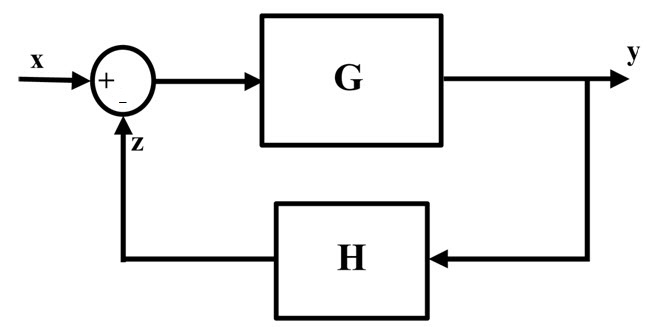
\includegraphics[scale=0.3]{plot.jpg}
\end{figure}
Closed loop gain Y(s)/X(s) = G(s)/1+G(s)H(s) \\
Open loop gain = G(s)


Therefore reduced gain

\end{frame}



\begin{frame}
Gain(db) Vs frequency \\

\begin{figure}
    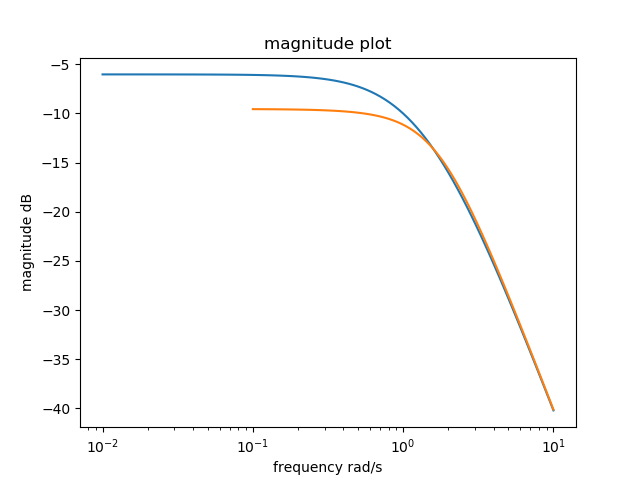
\includegraphics[scale=0.35]{plot2.png}
\end{figure}

So bandwidth increases


\end{frame}


\end{document}
